\documentclass[12pt]{beamer}

\usepackage{beamerthemeHannover, graphicx, clrscode, amsmath, amssymb, multicol}
\setbeamercolor{sidebar}{use=structure,bg=gray!20!green!60!white}

\title{Creating CPAN Modules with SWIG}
\author[J.A. Leto]{Jonathan Leto}
\date{}

\begin{document}
\frame{
    \titlepage
    \begin{center}
    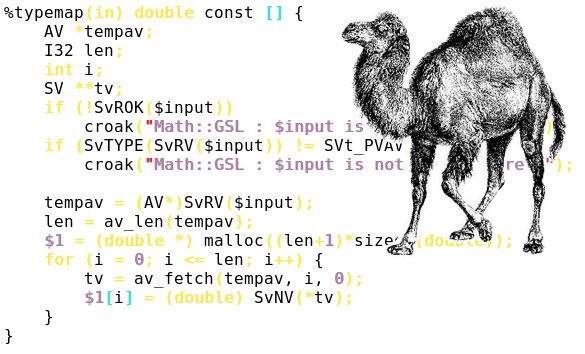
\includegraphics[width=5.84cm, height=3.85cm]{swig_camel}
    \end{center}
}

\section{Philosophy}
\frame{
    \frametitle{Don't Write Glue}
    \begin{center}
    \begin{columns}[t]
        \begin{column}{5cm}
            
\includegraphics[width=5.00cm, height=5.00cm]{xs_is_glue}
        \end{column}
        \begin{column}{5cm}
            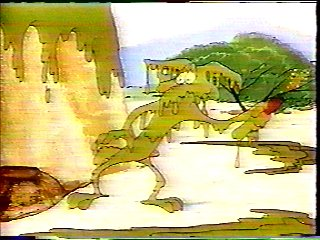
\includegraphics[width=5.00cm, height=5.00cm]{acmeglue}
        \end{column}
    \end{columns}
    \end{center}

}

\frame{
    \frametitle{Use an Integrating Pistol}
    \begin{center}
    
\includegraphics[width=6.26cm, height=3.70cm]{integrating_pistol}\\
    Need to integrate totally separate entities??\\
    Integrate it instantly with the ACME Integrating Pistol!!
    \end{center}
}
\section{Basics}
\subsection{Intro to XS}
\frame{
    \frametitle{What is XS?}
    \begin{itemize}
        \item eXternal Subroutine
        \item Large collection of macros which allow C/C++ method calls
        \item Extremely verbose 
            \begin{itemize}
                \item Math::GSL 0.10 has $\approx 274,000$ lines of XS
            \end{itemize}
        \item perldoc perlxs
    \end{itemize}
}
\subsection{Intro to SWIG}
\frame{
    \frametitle{What is SWIG?}
    \begin{itemize}
        \item Simplified Wrapper Interface Generator
        \item Creates a scripting language API to a C/C++ library 
        \item 18 target languages supported
        \item Reads header files and transforms datatypes between languages
        \item Automatic argument type checking
        \item Concise
            \begin{itemize}
                \item Math::GSL 0.10 has $\approx 500 $ lines of SWIG \\
                   which generates $\approx 274,000$ lines of XS
            \end{itemize}
    \end{itemize}
}
\subsection{Intro to Math::GSL}
\frame{
    \frametitle{What is Math::GSL?}
    \begin{itemize}
        \item Perl Interface to the GNU Scientific Library (GSL), which is written in C 
        \item Provides low-level access that emulates C calling style
        \item Also provides higher-level OO interface to some subsystems
        \item Broken into 48 subsystems like Vector, Matrix, RNG, Complex, Histogram, ... 
        \item Extensive tests (3279 as of 0.10)
    \end{itemize}
}
\subsection{Module::Build and SWIG}
\frame{
    \frametitle{Module::Build and SWIG}
    \begin{itemize}
        \item Module::Build does {\bf{not}} support SWIG directly
        \item Subclassing to the rescue!
    \end{itemize}
    \begin{center}
        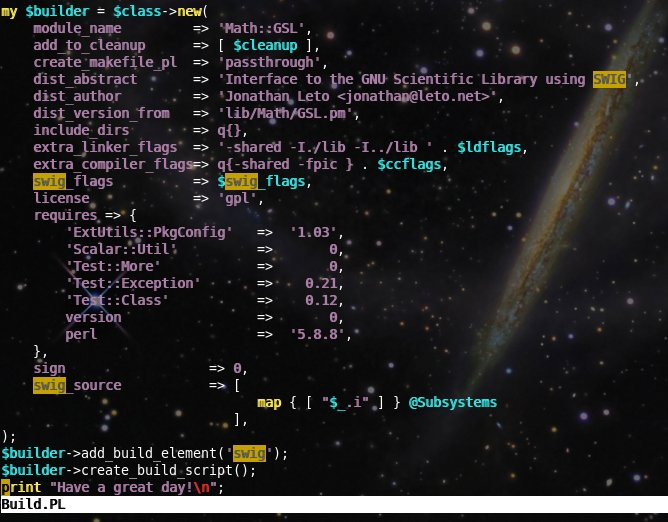
\includegraphics[width=8.00cm, height=5.00cm]{subclass}\\
    \end{center}
}
\frame{
    \frametitle{SWIG Example Code}
    \begin{center}
        ::begin vim hack session::\\
        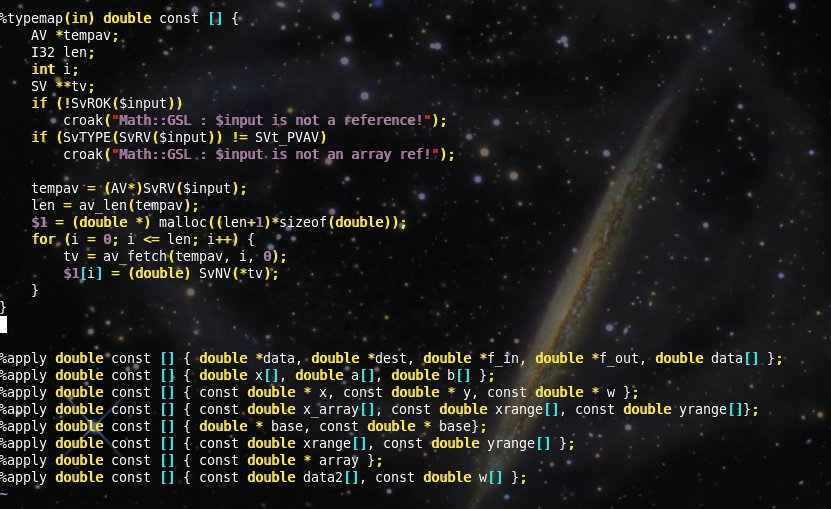
\includegraphics[width=8.00cm, height=5.00cm]{gsl_typemaps}\\
        ::end vim hack session::\\
    \end{center}
}
\section{Going Forward}

\frame{
    \frametitle{Active Development Continues}

    \begin{itemize}
        \item Scientific Computing applications built on top of Math::GSL
        \item Full gsl\_function callback support
        \item Static libraries and error handlers
        \item Porting to Darwin and Solaris
        \item Threads
    \end{itemize}
}
\section{Acknowledgements}
\frame{
    \frametitle{Thanks}

    \begin{itemize}
        \item Device::Cdio
        \item Thierry Moisan
        \item Eric Wilhelm
        \item \#pdx.pm
        \item Leslie Hawthorn
        \item The entire Google Summer of Code crew
    \end{itemize}
}

\frame{
    \frametitle{More Info}
    \begin{itemize}
        \item {http://www.swig.org}\\
        \item {http://leto.net/gitweb/}\\
        \item {http://leto.net/code/Math-GSL/}\\
        \item {http://groups.google.com/group/math-gsl-dev}\\
        \item {http://groups.google.com/group/perl-scientific-computing}\\
    \end{itemize}

}

\end{document}
